\documentclass{ximera}

% vier voorkeuren die je meteen zelf kan instellen:
\def\uitbr{0} % waarde 1 als je Uitbreiding in de marge wilt, 0 als je dat niet wilt 
\def\wsg{0} % waarde 1 als je verwijzingen naar Wiskunde Samen gevat² in de marge wilt, 0 als je dat niet wilt
\def\rectoverso{0} % waarde 1 als je het PDF-bestand recto-verso wilt laten afdrukken, 0 als je het recto wilt
\def\voetn{1} % waarde 1 als je de voetnoten wilt, 0 als je dat niet wilt 

% marges:
\usepackage[paper=a4paper,margin=3.4cm,marginparwidth=2cm]{geometry}

% packages algemeen:
\pdfOnly{
\usepackage[english,dutch]{babel}
}
\usepackage{amsfonts}
\usepackage{amsmath} %  o.a. \eqref en \text, omgeving equation*
\usepackage{amssymb} % o.a. \nmid
\usepackage{amsthm} % o.a. omgeving proof
\usepackage{graphicx} % o.a. figuren
\usepackage{xcolor} % \color
\usepackage[disable]{todonotes} % \todo 
\usepackage{comment} % omgeving comment
\usepackage{xcolor} % kleuren 
\usepackage[skip=7pt plus1pt, indent=0pt]{parskip} % skip = verticale ruimte tussen twee alinea's, indent = insprong bij nieuwe alinea
\usepackage{multicol} % kolommen
\usepackage{xfrac} % breuken

\usepackage{siunitx} % SI eenheden
\usepackage{eso-pic} % achtergrond voorpagina
\usepackage{tabularx} % kolommen voor rekenmachine
\usepackage{rotating} % voor omgeving turn

% voor figuren met PSTricks:
\usepackage{pstricks} 
\usepackage{pstricks-add}
\usepackage{pst-plot}
\usepackage{pst-node}
\usepackage{pst-coil}
\usepackage{auto-pst-pdf}

% voor figuren met TikZ:
\usepackage{tikz} 
\usepackage{tkz-euclide} 
\usepackage{pgfplots} 
\usetikzlibrary{calc,intersections,through,backgrounds,patterns} 
\pgfplotsset{compat=newest}
\usepgfplotslibrary{fillbetween,colormaps}
\usepackage{import}
\usepackage{tikz-3dplot}

% zelfde parskip in minipage:
\makeatletter
\setlength{\parskip}{\medskipamount}
\newcommand{\@minipagerestore}{\setlength{\parskip}{\medskipamount}}
\makeatother

% voor veranderen van de naam Bibliografie naar Referentielijst:
\pdfOnly{
\addto\captionsdutch{\renewcommand{\bibname}{Referentielijst}}

% voor trefwoordenlijst:
\usepackage{imakeidx}
\makeindex[title=Trefwoordenlijst,program=makeindex,options=-s index.tex,columns=2,intoc=true]
}
% voor nummeren van vergelijkingen:
%WIM%\numberwithin{equation}{chapter} % als je dit desactiveert dan worden vergelijkingen in bijvoorbeeld hoofdstuk 3 genummerd als (1), (2) etc. in plaats van (3.1), (3.2) etc.

% voor hyperlinks en bladwijzers in PDF-bestand:
%WIM%\usepackage[bookmarksopen,bookmarksopenlevel=0,hypertexnames=false,pdfa,bookmarksnumbered]{hyperref} 
%WIM%\usepackage{bookmark} 

% voor hyperlinks: 
\hypersetup{pdfborder={0 0 0}, pdfstartpage=1,linkbordercolor={1 0 0}}%pdfborder={0 0 0} is geen rand rond hyperlinks, pdfborder={1 1 1} wel

% korter commando voor displaystyle, om bijvoorbeeld breuken groter te drukken in doorlopende tekst: 
\newcommand{\D}{\displaystyle}

% (veel)gebruikte verzamelingen:
\newcommand\NN{\mathbb{N}} % verzameling van de natuurlijke getallen
\newcommand\QQ{\mathbb{Q}} % verzameling van de rationale getallen
\newcommand\RR{\mathbb{R}} % verzameling van de re\"ele getallen
\newcommand\ZZ{\mathbb{Z}} % verzameling van de gehele getallen

% (veel)gebruikte operatoren:
\def\co{\operatorname{co}} % coördinaat van een punt
\def\ggd{\operatorname{ggd}} % positieve grootste gemene deler van twee gehele getallen niet beide nul
\def\gr{\operatorname{gr}} % graad van een veelterm

% voor kleur grafieken (donkergroen):
\definecolor{graf}{RGB}{0,100,0} 

% voor lijsten: 
% \usepackage{enumerate}
%WIM%\usepackage[shortlabels]{enumitem} 
\setlist{topsep=0em, itemsep=-0.15em}

% voor small bullet:
\newcommand\sbullet[1][.5]{\mathbin{\vcenter{\hbox{\scalebox{#1}{$\bullet$}}}}}

% voor meer verticale ruimte tussen vergelijkingen in align
\addtolength{\jot}{0.1cm}

% voor meervoudige voetnoten:
\usepackage{fnpct}

% voor het onderdrukken van voetnoten als optie:
\usepackage{letltxmacro}
\LetLtxMacro\Oldfootnote\footnote
\newcommand{\EnableFootNotes}{%
  \LetLtxMacro\footnote\Oldfootnote%
}
\newcommand{\DisableFootNotes}{%
  \renewcommand{\footnote}[2][]{\relax}
}

% voor verticale lijn in de marge (uitbreiding):
\usepackage[framemethod=default]{mdframed}
\usepackage{marginnote}
\reversemarginpar
\ifthenelse{\uitbr < 1}{\definecolor{rood}{RGB}{255,255,255}}{\definecolor{rood}{RGB}{254,64,64}} %HEX: #fe4040
\mdfdefinestyle{uitbreiding}{%
    topline=false,
    rightline=false,
    bottomline=false,
    leftline=true,
    linecolor=rood,
    linewidth=5pt,
    rightmargin=0pt,
    skipabove=10pt,% ipv 3
    skipbelow=0pt,
    leftmargin=-25pt,
    innerleftmargin=20pt,
    innerrightmargin=0pt,
    innertopmargin=0pt,
    innerbottommargin=0pt%,
%	needspace=30pt %minimumhoogte vooraleer lijn wordt gesplitst
    }
\newenvironment{Uitbreiding}{
    \marginpar{
        \center
		\vspace{0.1cm}
		\vspace{7pt}
		\rotatebox{90}{\color{rood}\Large \bf Uitbreiding}
	}
    \begin{mdframed}[style=uitbreiding]
    }{\vspace{-0.05cm}
    \end{mdframed}
}


% omgevingen voor lemma, definitie, voorbeeld etc.:
\newtheoremstyle{mystyle}
    {0em} % Space above
    {0em} % Space below
    {\itshape} % Body font
    {} % Indent amount
    {\bfseries} % Theorem head font
    {.} % Punctuation after theorem head
    {.5em} % Space after theorem head
    {} % Theorem head spec (can be left empty, meaning `normal')
\theoremstyle{mystyle}
%WIM%\newtheorem{lemma}{Lemma}[chapter] % als je [chapter] desactiveert dan Voorbeeld 3 in plaats van Voorbeeld 5.3, als je [chapter] vervangt door [section] dan Voorbeeld 5.2.3 in plaats van Voorbeeld 5.3 
%\theoremstyle{definition} % als je dit activeert dan is wat in de omgeving staat niet cursief gedrukt
\newtheorem{oefening}[lemma]{Oefening}
\newtheorem{definitie}[lemma]{Definitie} 
\newtheorem{voorbeeld}[lemma]{Voorbeeld}
\newtheorem{eigenschap}[lemma]{Eigenschap} 
\newtheorem{stelling}[lemma]{Stelling} 
\newtheorem{gevolg}[lemma]{Gevolg} 
\newtheorem{afspraak}[lemma]{Afspraak} 
\newtheorem{werkwijze}[lemma]{Werkwijze}

% omgeving proof, aangepaste ruimte: 
\makeatletter
\renewenvironment{proof}[1][\proofname]{\par
  \vspace{-\topsep}% remove the space after the theorem
  \pushQED{\qed}%
  \normalfont
  \topsep0pt \partopsep0pt % no space before
  \trivlist
  \item[\hskip\labelsep
        \itshape
    #1\@addpunct{.}]\ignorespaces
}{%
  \popQED\endtrivlist\@endpefalse
  \addvspace{0pt plus 0pt} % no space after
}
\makeatother

% kaderstijlen uit SOHO Wiskunde Plantyn:
\colorlet{steunkleur}{black}
\colorlet{steunkleurlicht}{steunkleur!30!white}
\colorlet{steunkleurkader}{steunkleur!7!white}
\colorlet{steunkleurkaderlicht}{steunkleur!2!white}

\mdfdefinestyle{kaderstijl_vol_licht}
{skipabove=6pt, 
skipbelow=6pt, 
backgroundcolor=steunkleurkader,
linecolor=steunkleurlicht,
linewidth = 0.4pt, 
topline=true,
bottomline=true, 
rightline=true,
innerleftmargin=5pt,
innerrightmargin=5pt,
innertopmargin=5pt,
leftmargin=0cm,
rightmargin=0cm,
innerbottommargin=5pt,
needspace=30pt % minimumhoogte voor splitsen kader
}
\surroundwithmdframed[style=kaderstijl_vol_licht]{definitie}
\surroundwithmdframed[style=kaderstijl_vol_licht]{stelling}
\surroundwithmdframed[style=kaderstijl_vol_licht]{lemma}
\surroundwithmdframed[style=kaderstijl_vol_licht]{eigenschap}
\surroundwithmdframed[style=kaderstijl_vol_licht]{gevolg}

% voor omgevingen voor oefening en antwoord:
\newenvironment{Oefening}{%
    \begin{enumerate}[ 
    series=Oef,
    resume=Oef,
    leftmargin=1.78em,
    label={\bfseries\arabic*.},
    ref=\arabic*
    ]
    \item %
    }{%
    \end{enumerate}
}
\newenvironment{Antwoord}{%
    \begin{enumerate}[%
    series=Antw,
    resume=Antw,
    leftmargin=1.78em,
    label={\bfseries\arabic*.},
    ref=\arabic*
    ]
    \item %
    }{%
    \end{enumerate}
}

% als de omgeving Uitbreiding start met een kaderomgeving (definitie, stelling, eigenschap, lemma of gevolg) dan moet wat extra verticale ruimte voorzien worden, met het commando \uitbreidingstartmetkader:
\def\uitbreidingstartmetkader{\mbox{}\vspace{-0.205cm}}

% % voor schema van de staartdeling:
% \usepackage{stackengine}
% \setstackgap{S}{5pt}
% \stackMath\def\stackalignment{r}
% \newcommand{\myRule}[3][white]{\textcolor{#1}{\rule{#2}{#3}}}
% \let\ph\phantom % enkel voor tekst
% \newcommand{\mph}[1]{% enkel voor math mode
%     \mathcolor{white}{#1}%
% }
% \def\staartmin{\rule{0.25cm}{0.1mm}\myRule{0.3cm}{0.1mm}}
% \def\staartphmin{\myRule{0.25cm}{0.1mm}\myRule{0.3cm}{0.1mm}}
% \newcommand{\staartstreep}[1]{\rule{\widthof{$#1$}}{0.1mm}}
% \newcommand{\staartphstreep}[1]{\myRule{\widthof{$#1$}}{0.1mm}}

% voor kolommen met schema van Horner:
\newcommand{\kolbreed}{1.0cm}
\newcolumntype{H}{>{\centering\arraybackslash$} p{\kolbreed} <{$}}

% voor nieuw commando utikzdashed: onderlijn (zoals underline) maar dan met stippellijn:
\tikzset{
    cheating dash/.code args={on #1 off #2 ends #3}{%
        \csname tikz@addoption\endcsname{%
            \pgfgetpath\currentpath%
            \pgfprocessround{\currentpath}{\currentpath}%
            \csname pgf@decorate@parsesoftpath\endcsname{\currentpath}{\currentpath}%
            \pgfmathparse{max(#1-#3,0)}\let\dashphase=\pgfmathresult%
            \pgfmathparse{\csname pgf@decorate@totalpathlength\endcsname-#1+2*\dashphase}\let\rest=\pgfmathresult%
            \pgfmathparse{#1+#2}\let\onoff=\pgfmathresult%
            \pgfmathparse{max(floor(\rest/\onoff), 1)}\let\nfullonoff=\pgfmathresult%
            \pgfmathparse{max((\rest-\onoff*\nfullonoff)/\nfullonoff+#2, #2)}\let\offexpand=\pgfmathresult%
            \pgfsetdash{{#1}{\offexpand}}{\dashphase pt}}%
    },
    cheating dash per segment/.style args={on #1 off #2 ends #3}{
        /utils/exec=\csname tikz@options\endcsname,%
        decoration={show path construction,
            lineto code={\draw [cheating dash=on #1 off #2 ends #3] (\tikzinputsegmentfirst) -- (\tikzinputsegmentlast);},
            curveto code={\draw [cheating dash=on #1 off #2 ends #3] (\tikzinputsegmentfirst) .. controls (\tikzinputsegmentsupporta) and (\tikzinputsegmentsupportb) .. (\tikzinputsegmentlast);},
            closepath code={\draw [cheating dash=on #1 off #2 ends #3] (\tikzinputsegmentfirst) -- (\tikzinputsegmentlast);}
        },
        decorate,
    },
}
\newcommand{\utikzdash}[1]{%
    \tikz[baseline=(todotted.base)]{
        \node[inner sep=0pt,outer sep=1.5pt] (todotted) {#1};
        \draw[cheating dash per segment=on 2pt off 2pt ends 2pt, line width=0.4pt] (todotted.south west) -- (todotted.south east);
    }%
}%

\providecommand{\xmemph}[1]{\textit{#1}}

% voor nieuw commando underdashed: onderlijn met stippellijnen en ook het woord cursief zetten:
\newcommand{\underdashed}[1]{%
    {\em\utikzdash{\!#1\!}}%
}

% voor icoon TI-84 Plus met verwijzing naar filmpje:
\newcommand{\grmlink}{\raisebox{0cm}{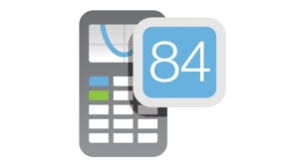
\includegraphics[width=1cm]{TI84Plus-icoon}}}
\newcommand{\grmref}[1]{%
	\reversemarginpar%
	\marginpar{
		\vspace{-0.4cm}%
		\htmladdnormallink{\grmlink}{#1}
	}	
}

% GRM knoppen:
\newcommand{\GRM}[1]{\fbox{\rule[0mm]{0cm}{0.215cm}\textup{\texttt{#1}}}}
\newcommand{\wedgetext}{{\raisebox{0.02cm}{\begin{turn}{90}>\end{turn}}}}
\newcommand{\veetext}{\raisebox{0.2cm}{\begin{turn}{-90}>\end{turn}}}

% voor kolommen met GRM screens:
\newlength{\widthallscreens}
\newlength{\widthscreens}
\newlength{\spaceleftscreen}
\newlength{\spacerightscreen}
\newlength{\spacebetweenscreens}

\newcommand{\setscreens}{
	\setlength{\spaceleftscreen}{2pt}
	\setlength{\spacerightscreen}{2pt}
	\setlength{\spacebetweenscreens}{8pt}
	\addtolength{\linewidth}{-28pt} % 3*8pt tussen vier screens en 2 pt links en 2 pt rechts
	\setlength{\widthallscreens}{\linewidth}
	\setlength{\widthscreens}{0.25\widthallscreens}
	\addtolength{\linewidth}{28pt}
	\newcolumntype{G}{p{\widthscreens}}
	\newcolumntype{s}{p{\spacebetweenscreens}}
	\newcolumntype{L}{p{\spaceleftscreen}}
	\newcolumntype{R}{p{\spacerightscreen}}
	\setlength{\tabcolsep}{0pt}
}

% voor icoon met verwijzing naar Wiskunde Samen gevat² in de marge:
% \newcommand{\wsglink}{\raisebox{0cm}{\includegraphics[width=1cm]{wsglogo}}}
\newcommand{\wsglink}{\raisebox{0cm}{LOGO}}
\newcommand{\htmladdnormallink}[2]{\href{#2}{#1}}
\newcounter{pagnrwsg}
\newcommand{\wsgref}[3]{% 
    % #1 woord dat onderstippeld wordt
    % #2 pagina van Wiskunde Samen gevat² waar je op terecht komt als je op de link klikt  
    % #3 afgedrukt op het logo van Wiskunde Samen gevat² in de marge: één of meerdere paginanummers
    \ifthenelse{\wsg < 1}{#1}{%
        \underdashed{#1}%
        {\setcounter{pagnrwsg}{#2}}%
        {\addtocounter{pagnrwsg}{14}}%
        \reversemarginpar%
        \marginpar{\vspace{-0.6cm}%
           \htmladdnormallink{\wsglink}{https://online.fliphtml5.com/sanky/laea/\#p=\arabic{pagnrwsg}}%
            \raisebox{0.41cm}[0cm][0cm]{%
                \hspace{-1.5cm}\makebox[2cm][c]{\colorbox{white}{\texttt{\footnotesize{#3}}}}%
            }%
        }%
    }%
}

% voor invoegen blanco pagina bij de optie recto-verso:
\def\blancobijrectoverso{
	\ifthenelse{\rectoverso < 1}{\clearpage}{
	\clearpage
	\thispagestyle{empty}
	\mbox{}
	\clearpage
	}
}

% aantal pagina's van het bestand:
\ifthenelse{\rectoverso < 1}{\def\totpag{57}}{\def\totpag{66}}

% documenteigenschappen:
% \usepackage{hyperxmp}
% \hypersetup{
% pdftitle={Open Source Wiskunde Aan zet: Veeltermen}, 
% pdfnumpages={\totpag},
% pdfauthor={Koen De Naeghel},
% pdflang={nl},
% pdfkeywords={wiskunde, open source, wiskunde aan zet, veeltermen, secundair onderwijs, tweede graad, doorstroomfinaliteit},
% pdfsubject={Veeltermen},
% pdfcopyright={\unichar{"24B8} 2024 Koen De Naeghel},
% pdfdate={17 december 2024},
% pdfapart=1,
% pdfstartview=}

% voor het benoemen van titel, auteur en datum:
% \title{Veeltermen}
% \author{Auteur: Koen De Naeghel}
% \date{\today}

\newcommand\BackgroundPic{
    \put(-260,-125){
    \parbox[b][\paperheight]{\paperwidth}{%
    \vfill
    \centering
    
\includegraphics[height=\paperwidth, keepaspectratio]{WaZlogo}%
    \vfill
}}}

\addPrintStyle{..}

\begin{document}
    \author{Kwinten Obbels}
    \xmtitle{Intro: een nieuwe soort getallen?}{}

Doorheen de geschiedenis van de wiskunde hebben nieuwe getallen een belangrijke rol gespeeld.
Uit het tellen komen de meest eenvoudige getallen voort: 1 appel, 2 appels, 3 appels, ... 
Dit zijn de natuurlijke getallen, die genoteerd worden met de letter \( \N = \{0, 1, 2, 3, 4, 5, 6, ...\} \) . 



Met deze getallen kan je op verschillende manieren 'nieuwe getallen' maken. 
Door negatieve getallen toe te voegen wordt de verzameling getallen groter.  
Dit zijn de gehele getallen, die genoteerd worden met de letter  \( \Z = \{0, +1,-1,+2,-2,+3,-3,+4,-4,+5,-5, ... \} \) . 


Één van de redenen waarom wiskundige nieuwe getallen invoeren, ligt in het oplossen van vergelijkingen. 
De vergelijking \(x + 7 = 0\) heeft geen oplossing in de natuurlijke getallen.
Zonder het gehele getal \(x = -7\) kan je deze vergelijking niet oplossen. 

%of: enkel het gehele getal x = -7 is een oplossing. 


\begin{denkvraag*}{}
    De Oude Grieken hebben negatieve getallen nooit aanvaard. 
    Voor hen is een getal altijd een hoeveelheid of een lengte, en dus positief. 
    \textbf{Ben jij akkoord met de Oude Grieken?}
    \\
\begin{tabular}{@{\qquad}l}
    Bestaan negatieve getallen wel 'écht'? \\
    Je hebt 1 appel, 2 appels, 3 appels, ... Maar wat is precies '-1 appel'? \\
    Aan welke vereisten moet iets voldoen voordat jij het 'een getal' zou willen noemen? \\
\end{tabular}
\end{denkvraag*}

\vspace{4mm}


Breuken leiden tot een volgende uitbreiding van de getallen.
%kunnen de gehele getallen \(\Z \) verder uitgebreid worden. 
Die nieuwe getallen worden de rationale getallen genoemd, en genoteerd met de letter \( \Q  = \left\{ \frac{z}{n} \mid z \in \Z, n \in \Nnul \right\}\).
Voorbeelden zijn \(\frac{2}{3}\), \(\frac{-4}{3}\), \(\frac{1}{1}\) en \(\frac{0}{3}\). 
Ook rationale getallen zijn nuttig om vergelijkingen op te lossen, 
want de vergelijking \(3x + 4 = 0\) heeft geen oplossing in de gehele getallen \( \Z \).
Zonder de breuk \(x = \frac{-4}{3}\) is deze vergelijking niet oplosbaar.

Je merkt al snel dat je nog niet 'genoeg' getallen hebt. 
De stelling van Pythagoras 
leert ons dat de schuine zijde van de gegeven driehoek lengte \( \sqrt{2}\) heeft. 


\begin{wrapfigure}{r}{3cm} 
    \begin{tikzpicture}[scale=2]
        % Define the vertices of the triangle
        \coordinate (A) at (0,0);
        \coordinate (B) at (1,0);
        \coordinate (C) at (0,1);
        % Draw the triangle
        \draw (A) -- (B) -- (C) -- cycle;
        
        % Label the hypotenuse with sqrt(2)
        \node at ($(B)!0.5!(C)$) [above right] {$\sqrt{2}$};
        \node at ($(A)!0.5!(B)$) [below] {$1$};
        \node at ($(A)!0.5!(C)$) [left] {$1$};
        
    \end{tikzpicture}
\end{wrapfigure}
    
Met een kort bewijs kan men aantonen dat \(\sqrt{2}\) niet in de verzameling rationale getallen zit, dus dat 
\[\sqrt{2} = 1.4142135623730950488016887242096980785696718753769480731766797\ldots%379907324784621070388503875343276...
\]  
niet te schrijven is als een breuk!. 
Deze getallen worden \textit{irrationaal} genoemd en hebben altijd oneindig veel cijfers na de komma.
%
Andere voorbeelden zijn 
\[ \pi = 3.141592653589793238462643383279502884197169399375\ldots%105820974944592307816406286208998628034825342117... 
,
\frac{\sqrt{2}}{2}
\Ten \pi^2 
\]
%
Ook irrationale getallen zijn nuttig om vergelijkingen op te lossen. 
De vergelijking \(x^2 + 2 = 4\) heeft immers geen oplossing in de rationale getallen \( \Q \).
Zonder het irrationale getal \(x = \sqrt{2} \) kan je deze vergelijking niet oplossen.
Als de irrationale getallen worden toegevoegd aan de rationale getallen \(\Q\), bekom je de reële getallen \(\R\). 
De reële getallen vormen een rechte waarbij met elk punt met een reëel getal overeenkomt. 

\begin{denkvraag*}{} 
    
    Bestaan er volgens jou nog andere soorten getallen? 
\begin{itemize}
    \item Zijn er vergelijkingen die je niet kan oplossen met de reële getallen \( \R \) ?
    \item Zou je de reële rechte nog kunnen 'uitbreiden'? 
    % \item Bestaat er volgens jou een 'oneindig' groot getal \( \infty \)? 
    % \item Bestaat het getal \(0.00\dots001 \) ? 
    
\end{itemize}
% \begin{tabular}{@{\qquad}l}
%     Bestaan er volgens jou nog andere soorten getallen? \\
%     Zijn er vergelijkingen die je niet kan oplossen met de reële getallen \( \R \)  \\
%     Zou je de reële rechte nog kunnen 'uitbreiden'?  \\
%     Bestaat er volgens jou een 'oneindig' groot getal (\infty\) \\
%     Bestaat het getal \(0.00\dots001 \) \\
% \end{tabular}
\end{denkvraag*}

\xmsection{Op zoek naar nieuwe getallen: een complexe geschiedenis...}

\begin{exercise}{Heron van Alexandrië}

    De Griekse wiskundige Heron van Alexandrië zocht in de eerste eeuw v. Chr de hoogte \(h\) van een afgeplatte piramide met basis b, afgeplatte top a en schuine ribbe c. 

    \textbf{a)} 
    Toon met behulp van de stelling van Pythagoras aan dat de hoogte h wordt gegeven door: \[h = \sqrt{c^2 - {\frac{b-a}{2}}^2}\]. 

    \textbf{b)} 
    Heron van Alexandrië berekende de hoogte van de afgeplatte piramide met volgende afmetingen: b = 28, a = 4 en c = 15. 
    \textbf{Ga Heron van Alexandrië achterna en voer deze berekening uit, valt er je iets op aan het eindresultaat? }
    
    \begin{image}[0.8\textwidth]
        
        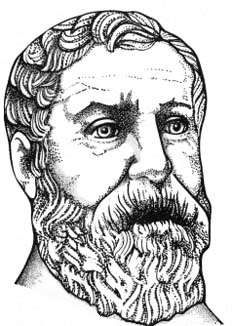
\includegraphics[width = 3cm]{portret_Heron.png}
        \(\qquad \qquad \qquad\)
        \begin{tikzpicture}

            % Define perspective transformation
            \tdplotsetmaincoords{70}{120}
            \begin{scope}[tdplot_main_coords]
            
            % Define the bottom base coordinates
            \coordinate (A) at (-2,-2,0);
            \coordinate (B) at (2,-2,0);
            \coordinate (C) at (2,2,0);
            \coordinate (D) at (-2,2,0);
            
            % Define the top base coordinates
            \coordinate (E) at (-1,-1,3);
            \coordinate (F) at (1,-1,3);
            \coordinate (G) at (1,1,3);
            \coordinate (H) at (-1,1,3);
            
            \coordinate (El) at (-1,-1,0);
            \coordinate (Fl) at (1,-1,0);
            \coordinate (Gl) at (1,1,0);
            \coordinate (Hl) at (-1,1,0);
            
            % Draw the solid edges
            \draw[thick, dashed] (A) -- (B);
            \draw[thick] (B) -- (C);
            \draw[thick] (C) -- node[below, blue]{\(b\)} (D) ;
            \draw[thick, dashed] (D) -- (A); % Bottom base
            
            
            \draw[thick] (E) -- (F) -- (G) -- node[above , blue, pos=0.3]{\(a\)} (H) -- cycle; % Top base
            \draw[dashed, brown, thick] (El) -- (Fl) -- (Gl) -- (Hl) -- cycle; % Top base
            \draw[thick, dashed] (A) -- (E);
            \draw[thick] (B) -- (F);
            \draw[thick] (C) -- (G);
            \draw[thick] (D) -- node[above right , blue, pos=0.4]{\(c\)} (H);
            
            % Draw the correct dashed lines (hidden edges)
            \draw[dashed, brown, thick] (H) -- node[left, blue, pos=0.5]{\(h\)}  (Hl); % Vertical hidden edge
            % \draw[dashed, brown, thick] (F) -- (Fl); % Vertical hidden edge
            
            \draw[dashed, brown, thick] (D) -- (Hl); % Vertical hidden edge
            
            
            \end{scope}
        \end{tikzpicture}

        
        
    \end{image}
    
    \captionof{figure}{Heron van Alexandrië en zijn afgeplatte piramide.}

\end{exercise}



\begin{denkvraag*}{}
\begin{itemize}
    \item Wat zou \(\sqrt{-4}\) kunnen betekenen? 
    \item Ken je een getal dat als kwadraat -4 heeft? 
    \item Zijn er vergelijkingen die \(\sqrt{-4}\) als oplossing hebben? 
\end{itemize}
\end{denkvraag*}


Heron van Alexandrië schreef als oplossing de positieve wortel \(\sqrt{63}\) in zijn schrift. 
Waarom hij dat deed is onduidelijk.
De meest voor de hand liggende verklaring is dat hij deze negatieve wortel niet kon aanvaarden. 

% \begin{wrapfigure}{o}{3cm} 
%     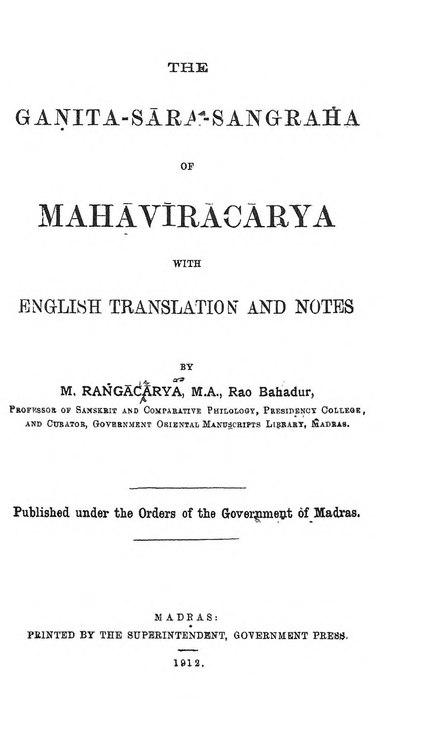
\includegraphics[width=4cm]{Indisch_boek.jpg}
% \end{wrapfigure}

In de 9de eeuw schreef de Indische wiskundige Mahaviracarya in zijn werk Ganita-Sara-Sangraha over wortels van negatieve getallen hetvolgende\footnote{
    David Eugene Smith, \textit{The Mathematics of Mahāvīrācārya with English Translations and Notes}, Bulletin of the American Mathematical Society, 1913, volume 19, p312. Eigen vertaling uit het Engels.} 

\begin{quote}
    'In de natuur der dingen is een negatieve hoeveelheid geen kwadraat, en het heeft dus geen vierkantswortel'.
\end{quote}
 

Het duurde tot de 16de eeuw voordat negatieve wortels opnieuw opdoken in de wiskunde, op het moment dat de Italiaanse wiskunde Cardano het volgende probleem probeerde op te lossen: 


\begin{exercise}{Gerolamo Cardano}

    Zoek 2 getallen waarvan de som gelijk is aan 10; en het product gelijk is aan 40.
    In symbolen is dit het stelsel \( 
        \begin{cases}
            x + y = 10 \\
            xy = 40
        \end{cases} \)
    waarbij \(x\) en \(y\) getallen zijn. \newline
    Cardano vond een oplossing voor dit probleem omdat hij rekende met negatieve wortels. \newline
    \textbf{Durf jij Cardono achterna om dit probleem op te lossen?}
\end{exercise}


Over zijn berekening schrijft Cardano zelf het volgende: 

\begin{quote}
    “Putting aside the mental tortures involved, 
    multiply \(5 + \sqrt{-15}\) and \(5 - \sqrt{-15}\) ... 
    Hence this product is 40... 
    This is truly sophisticated.”
\end{quote}

%TODO originale bron invoegen
%TODO nederlandse vertaling invoegen 



\begin{remark}
    Cardano heeft goede redenen om zijn negatieve wortels te omschrijven als 'mentale martelingen'.
    De rekenregel \(\sqrt{\square \square} = \sqrt{\square}\sqrt{\square}\) zorgt meteen voor een tegenstrijdigheid: 
    %underbrackets met -1 invoegen 
    \begin{center} 
        \textbf{We schrijven \(\sqrt{\square}\) enkel voor \( \square \in \R \)}. 
    \end{center}
\end{remark}


 
\begin{quickquestion*}{}
	Geef een voorbeeld van deze tegenstrijdigheid. 
\end{quickquestion*}


Om deze tegenstrijdige rekenregels te vermijden, voerde Euler een symbool \(i\) met als eigenschap dat \textbf{\(i^2 = -1\)}.
Het gebruik van negatieve wortels kan nu altijd vermeden worden: 

\[ \sqrt{-9} = \sqrt{-1 \cdot 9} = \sqrt{-1} \sqrt{9} = 3i  \]

{
\begin{wrapfigure}{r}{4cm} 
    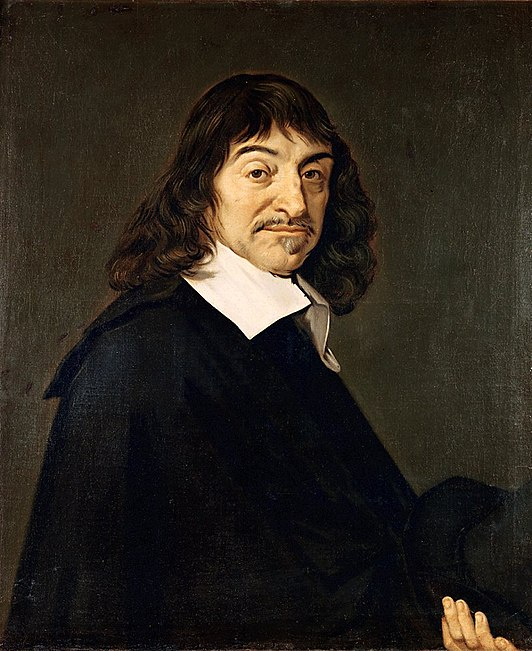
\includegraphics[width=3.5cm,keepaspectratio]{portret_Descartes.png}
    \captionof{figure}{René Descartes}
\end{wrapfigure}

René Descartes, bekend van het cartesiaans assenstelsel, is deze getallen tegengekomen bij het oplossen van meetkundige problemen. Hij schreef hierover\footnote{
    Descartes, René. \textit{La géométrie}. 1637, p47, Eigen vertaling uit het Frans.
    }: 
    
    
    
    
    \begin{quote}
        '...on ne fçaurait les rendre autres qu’ imaginaires.' 
        \\
        \\
    % \end{quote}
    % \begin{quote}
        '...we kunnen ze niet anders dan denkbeeldig maken.'
    \end{quote}
    
    
    Hierdoor is men deze nieuwe getallen 'imaginaire getallen' gaan noemen. 
    \vspace{2cm}
    
}

    %\newpage
    
    Om deze getallen beter te begrijpen zijn wiskundigen ze in een vlak beginnen voorstellen. Op de reële rechte stelt elk punt een reëel getal voor. In het \textbf{complexe vlak} zal elk punt een complex getal voorstellen. 
    
    
    
    De Ierse wiskundige William Rowan Hamilton schreef hierover in 1837 het volgende\footnote{
        Hamilton, William Rowan. \textit{Theory of Conjugate Functions or Algebraic
        Couples: with a Preliminary Essay on Algebra as a Science of Pure
        Time}, Irish Acad. Trans. \textbf{XVII} (1837), 519–422.}:   
    \begin{figure}[H]
        \centering
        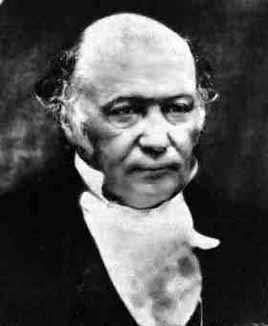
\includegraphics[width = 4cm,keepaspectratio]{portret_Hamilton.png}
        \caption{William Rowan Hamilton}
    \end{figure}

    \begin{quote}
        “...be concisely denoted as follows, \(\sqrt{-1} = (0, 1)\). In the theory of single numbers, the symbol \(\sqrt{-1}\) is absurd, and denotes an impossible extraction, or a merely imaginary number; but in the theory of couples, the same symbol \(\sqrt{-1}\) is significant, and denotes a possible extraction, or a real couple, namely the principal square-root of the couple \((-1,0)\).”
    \end{quote}
    
    %TODO nederlandse vertaling invoegen 
    

Uit het citaat blijkt dat in het vlak deze nieuwe getallen veel minder 'denkbeeldig' zijn dan wiskundigen lang gedacht hebben. Het nieuwe symbool \(i\) waarvoor \(i^2 = -1\),  blijkt simpelweg het punt \((0,1)\) te zijn. Omdat deze nieuwe getallen worden samengesteld uit het nieuwe symbool \(i\) en 2 reële getallen, kregen ze ook de naam 'complex'. 

Vandaag worden deze nieuwe 'complexe' getallen gebruikt bij het programmeren van computergames, bij het berekenen van elektronische schakelingen en in de kwantummechanica.

\end{document}